\pagestyle{fancy}
\fancypagestyle{plain}{}
\cfoot{\Roman{chapter}-\arabic{page}}
\rhead{}
\setcounter{page}{1}
\chapter{PENGEMBANGAN PERANGKAT LUNAK}

\section{Pendahuluan}
Dalam bab ini akan membahas tentang pengembangan perangkat lunak yang dilaksanakan
pada penelitian ini. Pengembangan perangkat lunak pada penilitian ini menggunakan metode \emph{Rational Unified Process} (RUP)
yang mana RUP terdiri dari empat fase yaitu fase insepsi, elaborasi, konstruksi, dan transisi.

\section{Fase Insepsi}~\label{fase_insepsi}
Pada fase insepsi terdiri dari langkah-langkah yang harus dilakukan yaitu pemodelan bisnis,
analisis data, mengidentifikasi kebutuhan pengguna, menentukan kebutuhan fungsional dan non-fungsional
dari perangkat lunak yang dikembangkan, dan yang terakhir adalah perancangan diagram \emph{use case}
dari perangkat lunak.

\subsection{Pemodelan Bisnis}~\label{insepsi_pemodelan_bisnis}
Hasil dari perangkat lunak yang dikembangkan pada penelitian ini dapat digunakan oleh pengguna
untuk melakukan analisis sentimen pada angkutan online untuk mengetahui seberapa puas konsumen
terhadap aplikasi angkutan online. Untuk mencapai tujuan tersebut maka penulis akan mengembangkan
perangkat lunak berbasis \emph{mobile} yang dapat melakukan analisis sentimen pada ulasan mengenai angkutan
online berbahasa Indonesia menggunakan metode CNN kedalam dua label yang tersedia yaitu positif dan
negatif. masukan yang diterima oleh perangkat lunak berupa kalimat dan file berkekstensi~.csv mengenai
angkutan online yang menghasilkan keluaran berupa probabilitas, dan label dari prediksi CNN
tersebut. Bentuk dari hasil pengembangan perangkat lunak dalam penelitian ini berupa
aplikasi \emph{mobile} dalam Sistem Operasi \emph{Android} menggunakan \emph{Kotlin}. \newpage

\pagestyle{fancy}
\fancypagestyle{plain}{}
\rhead{\Roman{chapter}-\arabic{page}}
\cfoot{}
\subsection{Kebutuhan Perangkat Lunak}
Fitur-fitur perangkat lunak yang dikembangkan ini berdasarkan pemodelan bisnis pada~\autoref{insepsi_pemodelan_bisnis}.
Perangkat lunak memiliki fitur-fitur utama yaitu memproses data teks berupa kalimat dan mengklasifikasikan
kalimat tersebut ke dalam label positif atau negatif. Kebutuhan fungsional adalah kebutuhan yang harus
ada pada perangkat lunak. Kebutuhan fungsional dari perangkat lunak yang dikembangkan dapat dilihat
pada Tabel~\ref{tab:kebutuhan_fungsional}.

\begin{table}[H]
  \centering
  \caption{Kebutuhan Fungsional Perangkat Lunak}
  \label{tab:kebutuhan_fungsional}
  \begin{tabularx}{\columnwidth}{|l|X|}
    \hline
    No & Kebutuhan Fungsional                                                                            \\ \hline
    1  & Perangkat lunak dapat menerima masukan berupa kalimat dan file berkestensi~.csv                 \\ \hline
    2  & Perangkat lunak dapat melakukan praproses pada kalimat yang akan dijadikan masukan ke model CNN \\ \hline
    3  & Perangkat lunak dapat menampilkan hasil klasifikasi berupa probabilitas dan labelnya            \\ \hline
  \end{tabularx}
\end{table}

Kebutuhan non-fungsional adalah kebutuhan yang tidak perlu ada pada perangkat lunak yang dikembangkan
namun akan sangat membantu jika ada. Kebutuhan non-fungsional pada perangkat lunak yang dikembangkan
dapat dilihat pada Tabel~\ref{tab:kebutuhan_nonfungsional}.

\begin{table}[H]
  \centering
  \caption{Kebutuhan Non-Fungsional Perangkat Lunak}
  \label{tab:kebutuhan_nonfungsional}
  \begin{tabularx}{\columnwidth}{|l|X|}
    \hline
    No & Kebutuhan Non-Fungsional                                             \\ \hline
    1  & Perangkat lunak memiliki antarmuka yang mudah dipahami oleh pengguna \\ \hline
  \end{tabularx}
\end{table}

\subsection{Analisis Perangkat Lunak}
Dari pembahasan pada pemodelan bisnis dapat diperoleh apa saja yang diharapkan oleh pengguna dari
perangkat lunak yang dikembangkan yaitu sebagai berikut.
\begin{itemize}
  \item Menerima masukan data berupa kalimat pada \emph{text field}.
  \item Menerima masukan data berupa file berkestensi~.csv.
  \item Melakukan praproses pada masukan.
  \item Melakukan analisis sentimen dengan menggunakan model CNN\@.
\end{itemize}

\subsection{Desain Perangkat Lunak}
Pada bagian ini akan menjelaskan secara detil tentang diagram \emph{use case}, tabel definisi aktor, tabel
definisi \emph{use case}, dan tabel skenario \emph{use case}.

\subsubsection{Diagram \emph{Use Case}}
\emph{Use case} diagram adalah proses pengilustrasian yang dilakukan pengguna atau aktor untuk menunjukkan hubungan
antara pengguna atau aktor terhadap perangkat lunak yang dikembangkan. \emph{Use case} diagram dapat dilihat
pada Gambar~\ref{fig:usecase_diagram}.

\begin{figure}[H]
  \centering
  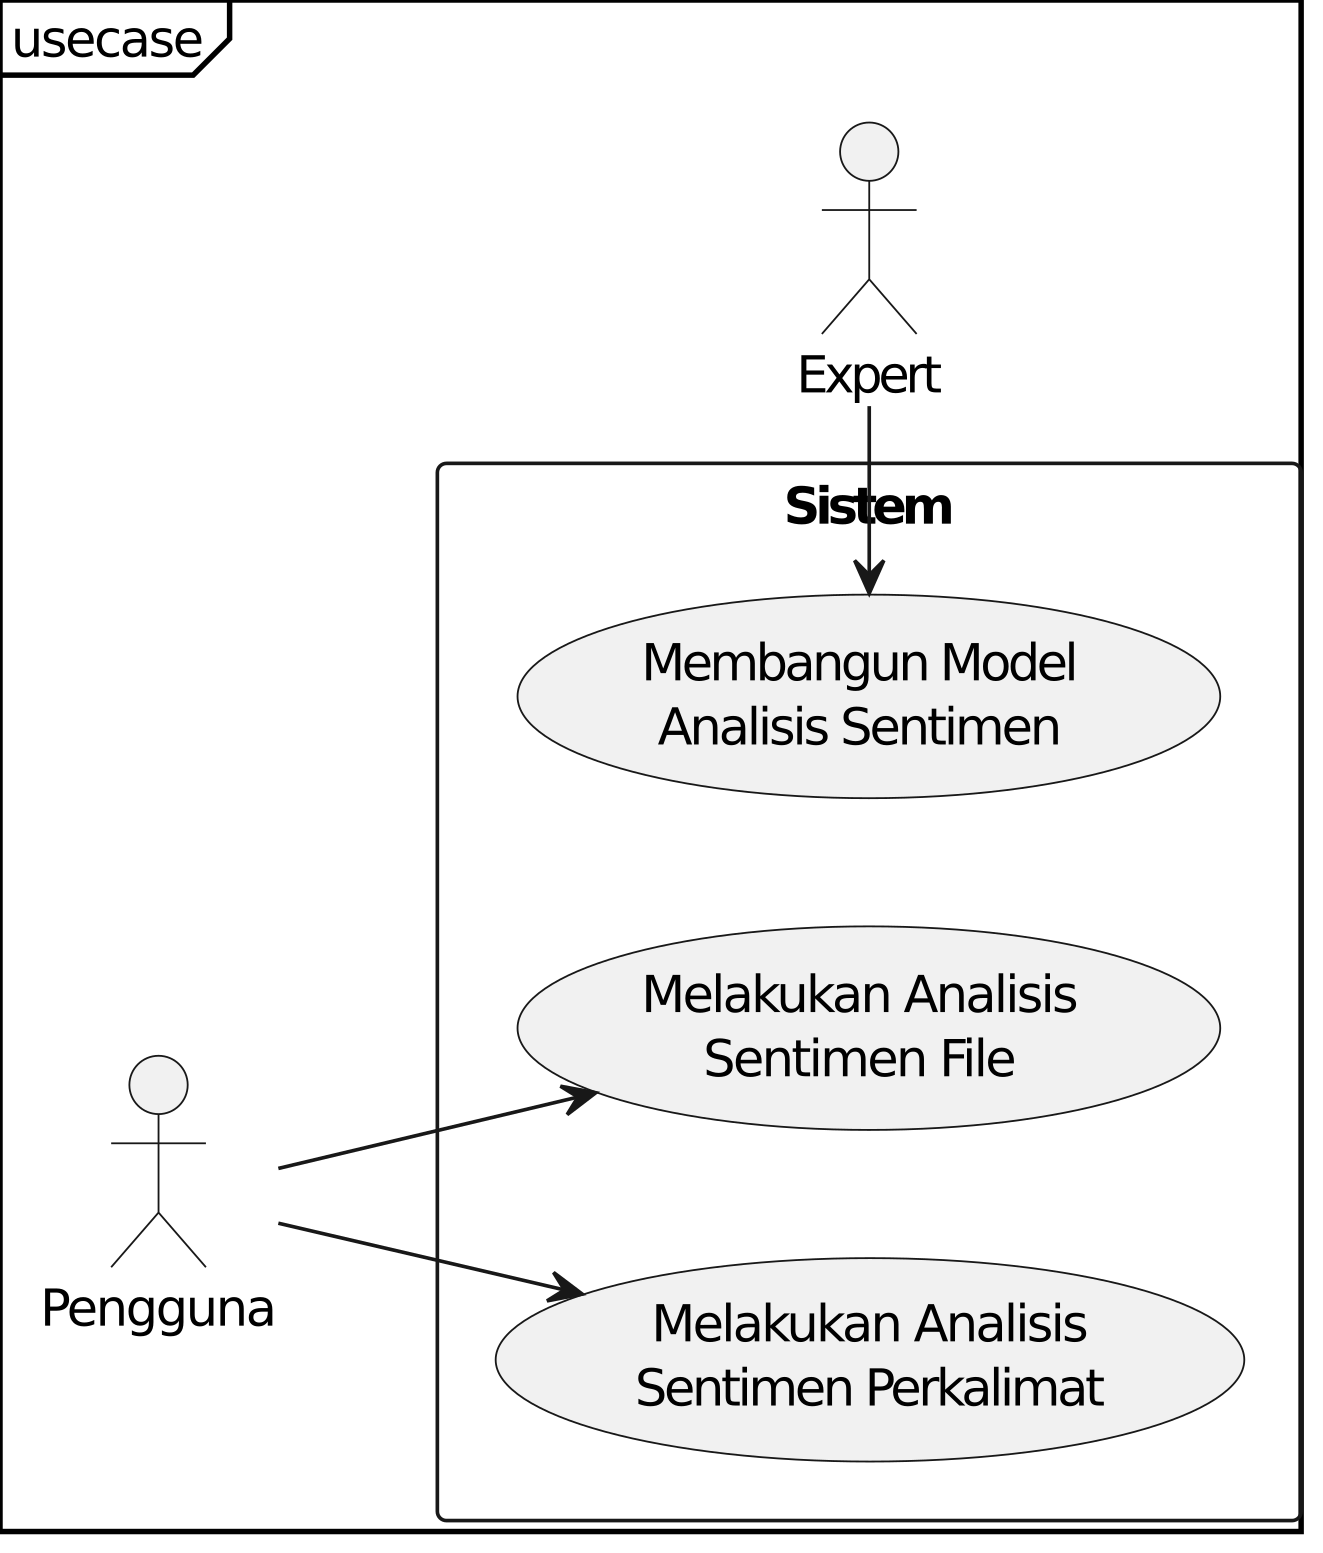
\includegraphics[scale=1]{assets/usecase_diagram.png}
  \caption{Diagram \emph{Use Case}}
  \label{fig:usecase_diagram}
\end{figure}

\subsubsection{Definisi \emph{Use Case}}
Penjelasan lebih detail dari diagram \emph{use case} pada Gambar~\ref{fig:usecase_diagram} diatas dapat dilihat
pada Tabel~\ref{tab:definisi_usecase}.

\begin{table}[H]
  \centering
  \caption{Definisi \emph{Use Case}}
  \label{tab:definisi_usecase}
  \begin{tabularx}{\textwidth}{|l|l|X|}
    \hline
    No & Use Case                        & Keterangan \\ \hline
    1  & \makecell[l]{Melakukan Analisis              \\Sentimen Kalimat} & Salah satu fitur utama dari aplikasi dimana sistem akan menerima masukan berupa kalimat dan menampilkan hasil dari operasi analisis sentimen           \\ \hline
    2  & \makecell[l]{Melakukan Analisis              \\Sentimen File}    & Salah satu fitur utama dari aplikasi dimana sistem akan menerima masukan berupa file berkekstensi~.csv dan menampilkan hasil operasi analisis sentimen \\ \hline
    3  & \makecell[l]{Membangun Model                 \\Analisis Sentimen}    & Dalam usecase ini dilakukan pelatihan model CNN untuk melakukan analisis sentimen dan pengukuran kinerja dari model dengan menggunakan data uji\\ \hline
  \end{tabularx}
\end{table}

\subsubsection{Definisi Aktor}
Aktor merupakan seseorang yang berinteraksi dengan \emph{use case} melalui perangkat lunak yang dikembangkan.
Penjelasan tentang aktor dapat dilihat pada Tabel~\ref{tab:aktor_definisi}.

\begin{table}[H]
  \centering
  \caption{Definisi Aktor}
  \label{tab:aktor_definisi}
  \begin{tabularx}{\columnwidth}{|l|l|X|}
    \hline
    No & Aktor    & Definisi                                                                                                          \\ \hline
    1  & Pengguna & Pengguna adalah seseorang yang ingin menggunakan semua fitur yang terdapat pada perangkat lunak yang dikembangkan \\ \hline
    2  & Expert   & Expert adalah seseorang yang membangun dan mengukur kinerja dari model CNN untuk melakukan analisis sentimen      \\ \hline
  \end{tabularx}
\end{table}

\subsubsection{Skenario \emph{Use Case}}
Skenario \emph{use case} adalah alur dari proses \emph{use case} dari sisi aktor dan sistem.
Setiap \emph{use case} yang ada pada diagram memiliki skenario. Penjelasan tentang skenario untuk setiap
\emph{use case} dapat dilihat pada Tabel~\ref{tab:scenario_usecase_kalimat},~\ref{tab:scenario_usecase_file},~\ref{tab:scenario_usecase_train}.

\begin{longtable}[c]{|ll|}
  \caption{Skenario Usecase Analisis Sentimen Kalimat}
  \label{tab:scenario_usecase_kalimat}                                                                                                                                                                                                                         \\
  \hline
  \multicolumn{2}{|c|}{\textbf{Identifikasi}}                                                                                                                                                                                                                  \\ \hline
  \endhead
  %
  \multicolumn{1}{|l|}{\textbf{Nomor}}                                                                            & UC-01                                                                                                                                      \\ \hline
  \multicolumn{1}{|l|}{\textbf{Nama}}                                                                             & Melakukan analisis sentimen perkalimat                                                                                                     \\ \hline
  \multicolumn{1}{|l|}{\textbf{Aktor}}                                                                            & Pengguna                                                                                                                                   \\ \hline
  \multicolumn{1}{|l|}{\textbf{Tujuan}}                                                                           & Menampilkan hasil dari analisis sentimen                                                                                                   \\ \hline
  \multicolumn{1}{|l|}{\textbf{Deksripsi}}                                                                        &
  \begin{tabular}[c]{@{}l@{}}Dalam usecase ini dilakukan analisis sentimen\\ pada kalimat yang dimasukkan ke text box oleh\\ pengguna  sebagai masukan. Kalimat akan\\ dilakukan klasifikasi menggunakan model yang \\ telah dilatih oleh expert.\end{tabular} \\ \hline
  \multicolumn{1}{|l|}{\textbf{Kondisi Awal}}                                                                     &
  \begin{tabular}[c]{@{}l@{}}Pengguna memasukan data ke text box yang \\ ada di aplikasi android\end{tabular}                                                                                                                                                  \\ \hline
  \multicolumn{2}{|c|}{\textbf{Skenario Normal}}                                                                                                                                                                                                               \\ \hline
  \multicolumn{1}{|l|}{\textbf{Aktor}}                                                                            & \textbf{Sistem}                                                                                                                            \\ \hline
  \multicolumn{1}{|l|}{\begin{tabular}[c]{@{}l@{}}1. Memilih Tab \\ Analisis Sentimen \\ Perkalimat\end{tabular}} &
  \begin{tabular}[c]{@{}l@{}}2. Menampilkan Analisis \\ Sentimen Perkalimat\end{tabular}                                                                                                                                                                       \\ \hline
  \multicolumn{1}{|l|}{}                                                                                          & \begin{tabular}[c]{@{}l@{}}3. Menerima Masukan\\ Berupa Kalimat\end{tabular}                                                               \\ \hline
  \multicolumn{1}{|l|}{}                                                                                          & \begin{tabular}[c]{@{}l@{}}4. Mengklasifikasi Sentimen\\ Positif Atau Negatif\end{tabular}                                                 \\ \hline
  \multicolumn{1}{|l|}{}                                                                                          & \begin{tabular}[c]{@{}l@{}}5. Menampilkan\\ Hasil Klasifikasi\end{tabular}                                                                 \\ \hline
  \multicolumn{1}{|l|}{\textbf{Kondisi Akhir}}                                                                    & \begin{tabular}[c]{@{}l@{}}Sistem menampilkan\\ hasil analisis sentimen\end{tabular}                                                       \\ \hline
\end{longtable}

\begin{longtable}[c]{|ll|}
  \caption{Skenario Usecase Analisis Sentimen File}
  \label{tab:scenario_usecase_file}                                                                                                                                                                                                                                                                                                             \\
  \hline
  \multicolumn{2}{|c|}{\textbf{Identifikasi}}                                                                                                                                                                                                                                                                                                   \\ \hline
  \endhead
  %
  \multicolumn{1}{|l|}{\textbf{Nomor}}                                                                  &
  UC-02                                                                                                                                                                                                                                                                                                                                         \\ \hline
  \multicolumn{1}{|l|}{\textbf{Nama}}                                                                   &
  Melakukan analisis sentimen file                                                                                                                                                                                                                                                                                                              \\ \hline
  \multicolumn{1}{|l|}{\textbf{Aktor}}                                                                  &
  Pengguna                                                                                                                                                                                                                                                                                                                                      \\ \hline
  \multicolumn{1}{|l|}{\textbf{Tujuan}}                                                                 &
  Menampilkan hasil dari analisis sentimen                                                                                                                                                                                                                                                                                                      \\ \hline
  \multicolumn{1}{|l|}{\textbf{Deksripsi}}                                                              &
  \begin{tabular}[c]{@{}l@{}}Dalam usecase ini dilakukan analisis sentimen \\ pada file berekstensi .csv yang berisi sentimen\\ sentimen dengan tiga kolom yang terdiri dari indeks,\\ sentimen, dan label oleh pengguna sebagai masukan.\\ Kalimat akan dilakukan klasifikasi menggunakan\\ model yang telah dilatih oleh expert.\end{tabular} \\ \hline
  \multicolumn{1}{|l|}{\textbf{Kondisi   Awal}}                                                         &
  \begin{tabular}[c]{@{}l@{}}Pengguna memasukan data ke text box yang ada \\ di aplikasi android\end{tabular}                                                                                                                                                                                                                                   \\ \hline
  \multicolumn{2}{|l|}{\textbf{Skenario Normal}}                                                                                                                                                                                                                                                                                                \\ \hline
  \multicolumn{1}{|l|}{\textbf{Aktor}}                                                                  &
  \textbf{Sistem}                                                                                                                                                                                                                                                                                                                               \\ \hline
  \multicolumn{1}{|l|}{\begin{tabular}[c]{@{}l@{}}1. Memilih tab analisis\\ sentimen file\end{tabular}} &
  2. Menampilkan analisis sentimen file                                                                                                                                                                                                                                                                                                         \\ \hline
  \multicolumn{1}{|l|}{}                                                                                &
  \begin{tabular}[c]{@{}l@{}}3. Menerima masukan berupa file berkestensi .csv\\ yang memiliki tiga kolom yang terdiri dari indeks,\\ sentimen, dan label\end{tabular}                                                                                                                                                                           \\ \hline
  \multicolumn{1}{|l|}{}                                                                                &
  4. Mengklasifikasi sentimen positif atau negatif                                                                                                                                                                                                                                                                                              \\ \hline
  \multicolumn{1}{|l|}{}                                                                                &
  5. Menampilkan hasil klasifikasi                                                                                                                                                                                                                                                                                                              \\ \hline
  \multicolumn{1}{|l|}{\textbf{Kondisi   Akhir}}                                                        &
  Sistem menampilkan hasil analisis sentimen                                                                                                                                                                                                                                                                                                    \\ \hline
\end{longtable}

\begin{longtable}[c]{|ll|}
  \caption{Skenario Usecase Analisis Sentimen Pelatihan}
  \label{tab:scenario_usecase_train}                                                                                                                                                                                                                                                                                                                                                 \\
  \hline
  \multicolumn{2}{|c|}{\textbf{Identifikasi}}                                                                                                                                                                                                                                                                                                                                        \\ \hline
  \endhead
  %
  \multicolumn{1}{|l|}{\textbf{Nomor}}                                                        &
  UC-03                                                                                                                                                                                                                                                                                                                                                                              \\ \hline
  \multicolumn{1}{|l|}{\textbf{Nama}}                                                         &
  Membangun model CNN untuk melakukan analisis sentimen                                                                                                                                                                                                                                                                                                                              \\ \hline
  \multicolumn{1}{|l|}{\textbf{Aktor}}                                                        &
  Expert                                                                                                                                                                                                                                                                                                                                                                             \\ \hline
  \multicolumn{1}{|l|}{\textbf{Tujuan}}                                                       &
  \begin{tabular}[c]{@{}l@{}}Menampilkan kinerja model CNN berupa akurasi, presisi, \\ recall  dan f1-score\end{tabular}                                                                                                                                                                                                                                                             \\ \hline
  \multicolumn{1}{|l|}{\textbf{Deksripsi}}                                                    &
  \begin{tabular}[c]{@{}l@{}}Dalam usecase ini dilakukan pelatihan model CNN untuk \\ melakukan analisis sentimen dengan menggunakan data\\ latih  dengan jumlah 3600 yang terdiri dari 1800 label positif\\ dan 1800 label negatif dan di validasi dengan  menggunakan\\ data validasi yang berjumlah 1200 yang terdiri dari 600 label\\ positif dan 600 label negatif\end{tabular} \\ \hline
  \multicolumn{1}{|l|}{\textbf{Kondisi Awal}}                                                 &
  Google Colab dalam kondisi belum tereksekusi                                                                                                                                                                                                                                                                                                                                       \\ \hline
  \multicolumn{2}{|c|}{\textbf{Skenario Normal}}                                                                                                                                                                                                                                                                                                                                     \\ \hline
  \multicolumn{1}{|l|}{\textbf{Aktor}}                                                        &
  \textbf{Sistem}                                                                                                                                                                                                                                                                                                                                                                    \\ \hline
  \multicolumn{1}{|l|}{\begin{tabular}[c]{@{}l@{}}1. Menekan\\ Tombol\\ Run All\end{tabular}} &
  2. Melakukan praproses pada teks                                                                                                                                                                                                                                                                                                                                                   \\ \hline
  \multicolumn{1}{|l|}{}                                                                      &
  3. Mengubah kata menjadi word embedding                                                                                                                                                                                                                                                                                                                                            \\ \hline
  \multicolumn{1}{|l|}{}                                                                      &
  4. Melakukan pelatihan model                                                                                                                                                                                                                                                                                                                                                       \\ \hline
  \multicolumn{1}{|l|}{}                                                                      &
  5. Menyimpan model yang telah dilatih                                                                                                                                                                                                                                                                                                                                              \\ \hline
  \multicolumn{1}{|l|}{}                                                                      &
  6. Menampilkan laporan hasil klasifikasi                                                                                                                                                                                                                                                                                                                                           \\ \hline
  \multicolumn{1}{|l|}{\textbf{Kondisi Akhir}}                                                &
  Sistem menampilkan hasil analisis sentimen                                                                                                                                                                                                                                                                                                                                         \\ \hline
\end{longtable}

\section{Fase Elaborasi}
Fase kedua atau fase elaborasi dalam fase ini terdapat aktivitas yang dilakukan yaitu pemodelan bisinis, perancangan antarmuka
pengguna atau \emph{user interface}, dan pembuatan \emph{sequence diagram}.

\subsection{Pemodelan Bisnis}
Pemodelan bisnis pada fase ini adalah melakukan perancangan perangkat lunak berdasarkan fase insepsi yang telah dilakukan
pada \autoref{fase_insepsi} sebelumnya. Perancangan yang dilakukan yaitu antarmuka () dan pembuatan
\emph{sequence diagram}.

\subsection{Perancangan Antarmuka (\emph{Interface})}
Terdapat dua halaman rancangan yang dibuat berdasarkan pada Fase Insepsi sebelumnya. Desain antarmuka
dapat dilihat pada Gambar~\ref{fig:rancangan_interface_kalimat} dan Gambar~\ref{fig:rancangan_interface_file}

\begin{figure}[H]
  \centering
  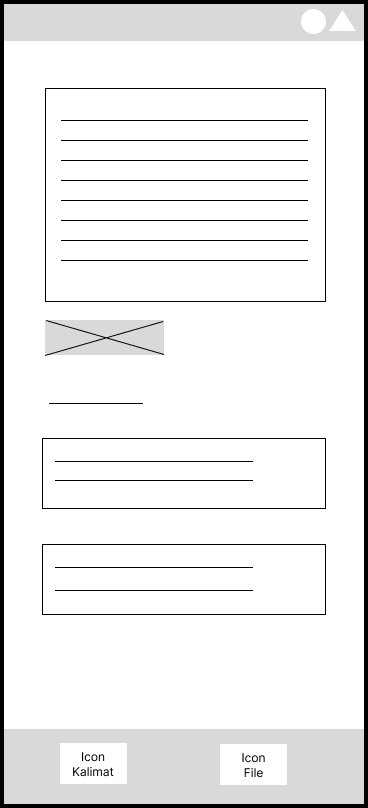
\includegraphics[width=4cm, height=8cm]{assets/rancangan_interface_kalimat.png}
  \caption{Rancangan Antarmuka Kalimat}
  \label{fig:rancangan_interface_kalimat}
\end{figure}

\begin{figure}[H]
  \centering
  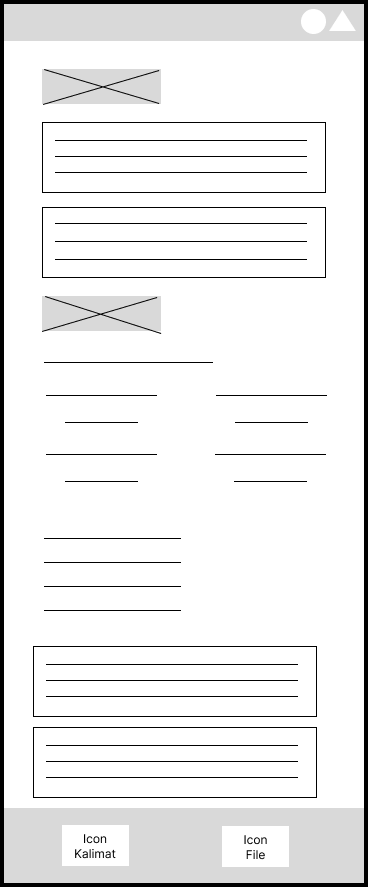
\includegraphics[width=4cm, height=8cm]{assets/rancangan_interface_file.png}
  \caption{Rancangan Antarmuka File}
  \label{fig:rancangan_interface_file}
\end{figure}

\subsection{Diagram Aktivitas}
Diagram aktivitas digunakan untuk mengilustrasikan alur kegiatan atau aktivitas dari sebuah
perangkat lunak yang dikembangkan sesuai pada pemodelan proses bisnis. Diagram aktivitas dapat dilihat
pada Gambar~\ref{fig:activity_diagram_kalimat} dan pada Gambar~\ref{fig:activity_diagram_file}.

\begin{figure}[H]
  \centering
  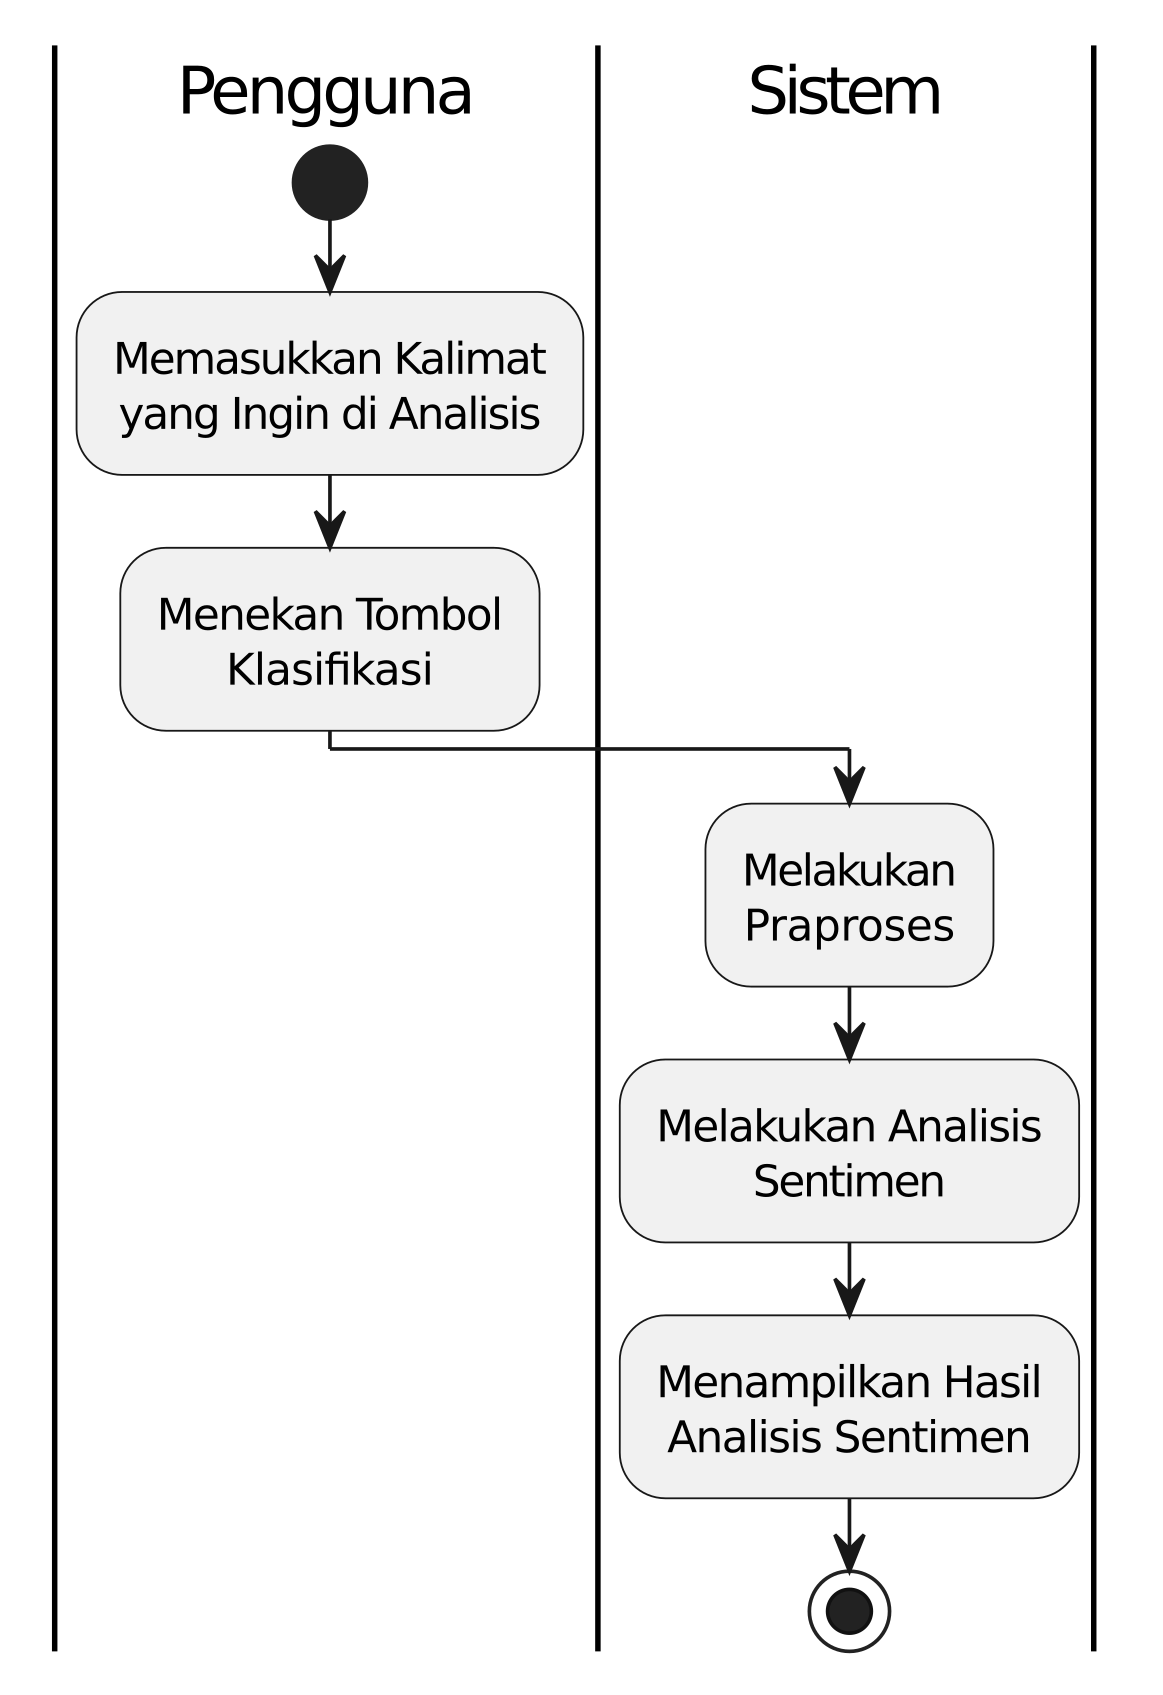
\includegraphics[scale=0.7]{assets/activity_diagram_kalimat.png}
  \caption{Diagram Aktivitas Kalimat}
  \label{fig:activity_diagram_kalimat}
\end{figure}

\begin{figure}[H]
  \centering
  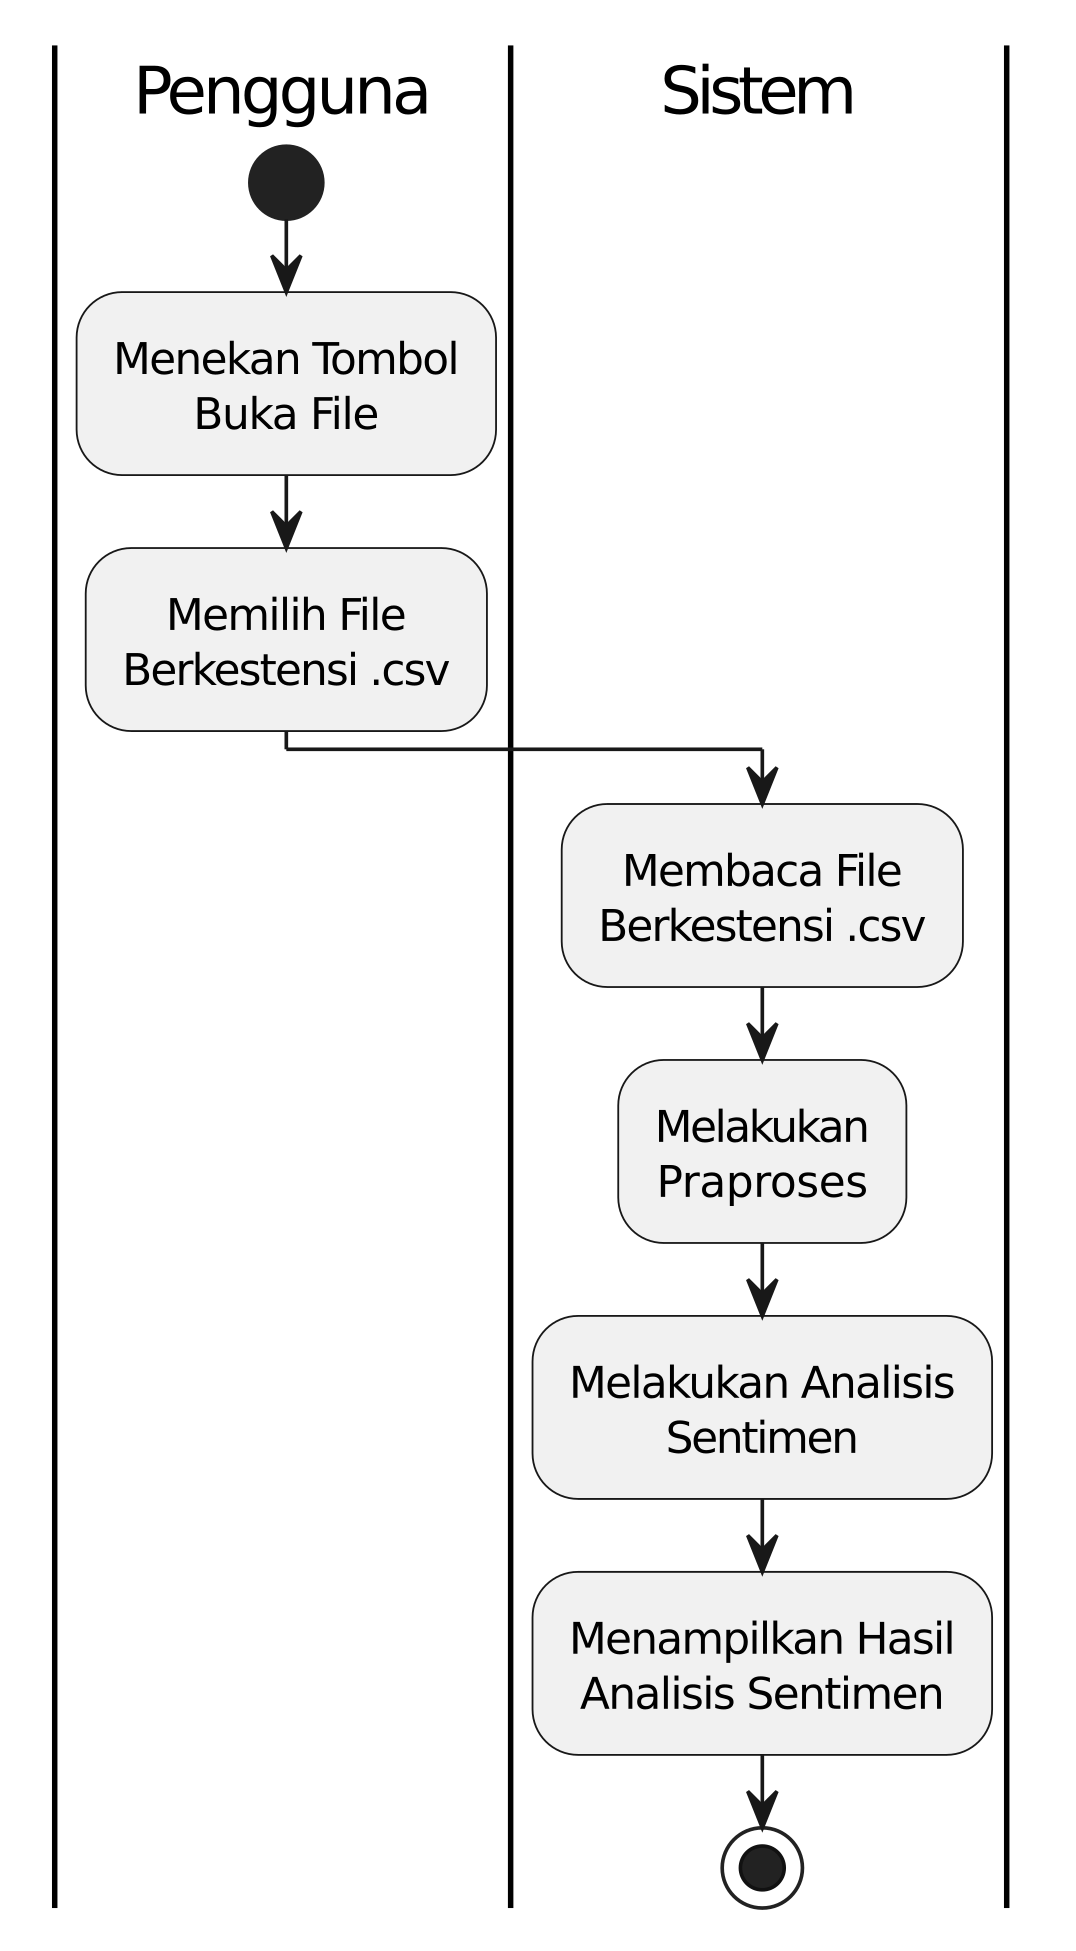
\includegraphics[scale=0.7]{assets/activity_diagram_file.png}
  \caption{Diagram Aktivitas File}
  \label{fig:activity_diagram_file}
\end{figure}

\begin{figure}[H]
  \centering
  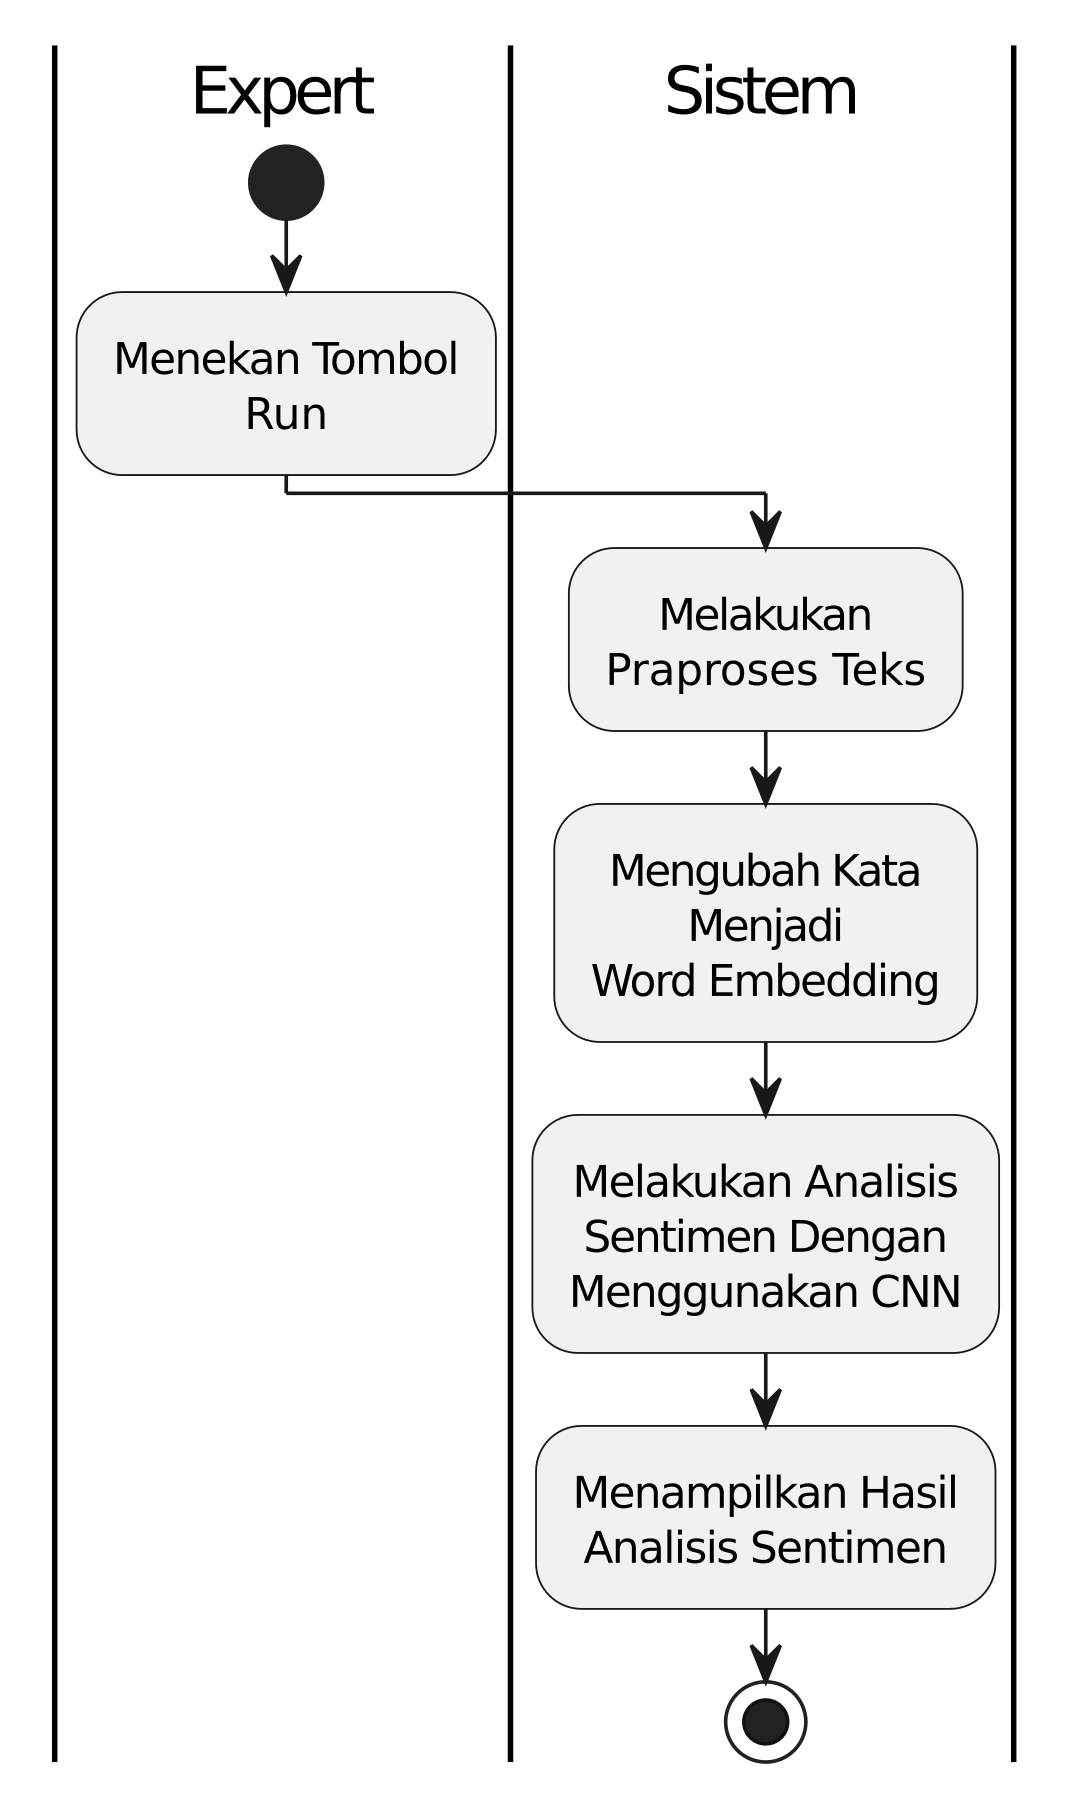
\includegraphics[scale=0.7]{assets/activity_diagram_test.png}
  \caption{Diagram Aktivitas Pengujian}
  \label{fig:activity_diagram_kalimat}
\end{figure}

\subsection{\emph{Sequence Diagram}}
Pada Sub Bagian \emph{Sequence Diagram} ini akan dijelaskan alur interaksi pada setiap objek didalam
perangkat lunak berdasarkan \emph{Use Case} yang telah dirancang. \emph{Sequence diagram} dapat dilihat
pada Gambar~\ref{fig:sequence_diagram_kalimat} dan Gambar~\ref{fig:sequence_diagram_file}.

\begin{figure}[H]
  \centering
  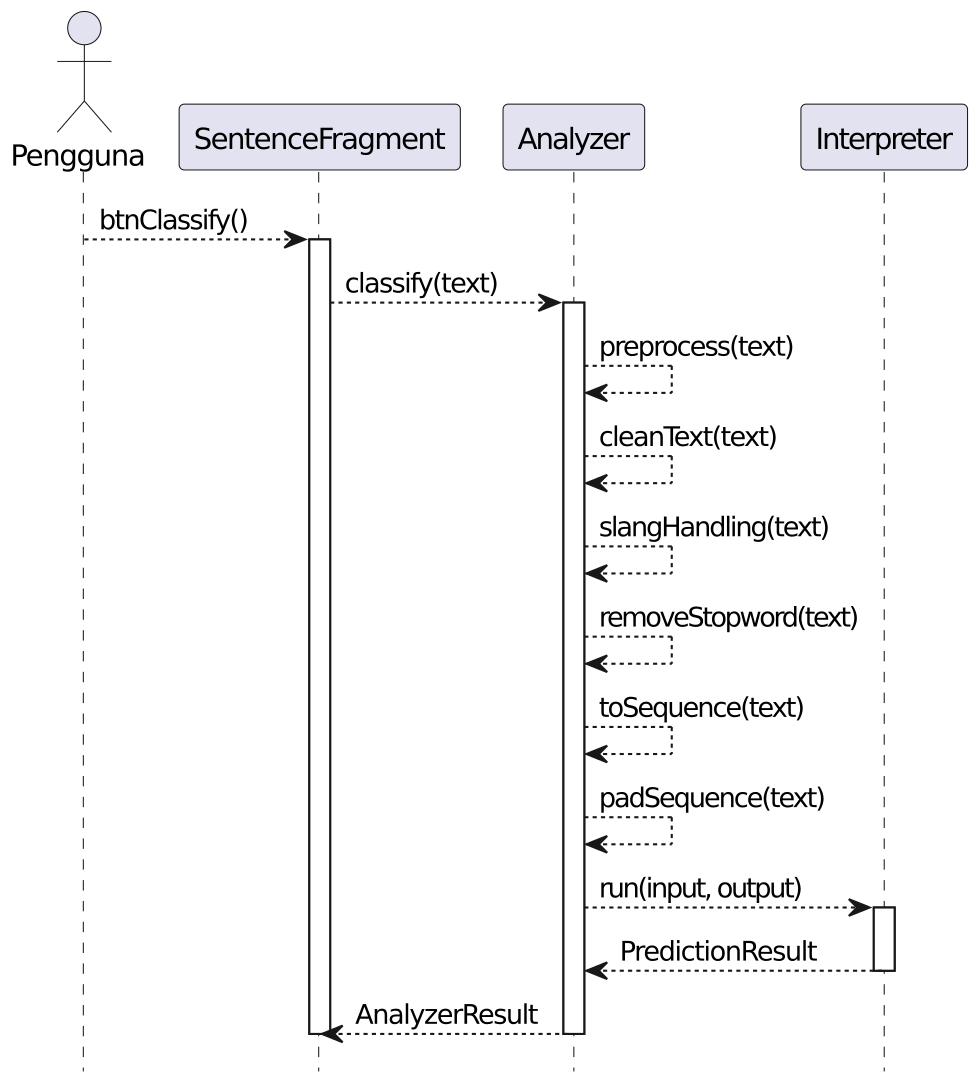
\includegraphics[width=\textwidth]{assets/sequence_diagram_kalimat.png}
  \caption{Sequence Diagram Kalimat}
  \label{fig:sequence_diagram_kalimat}
\end{figure}

\begin{figure}[H]
  \centering
  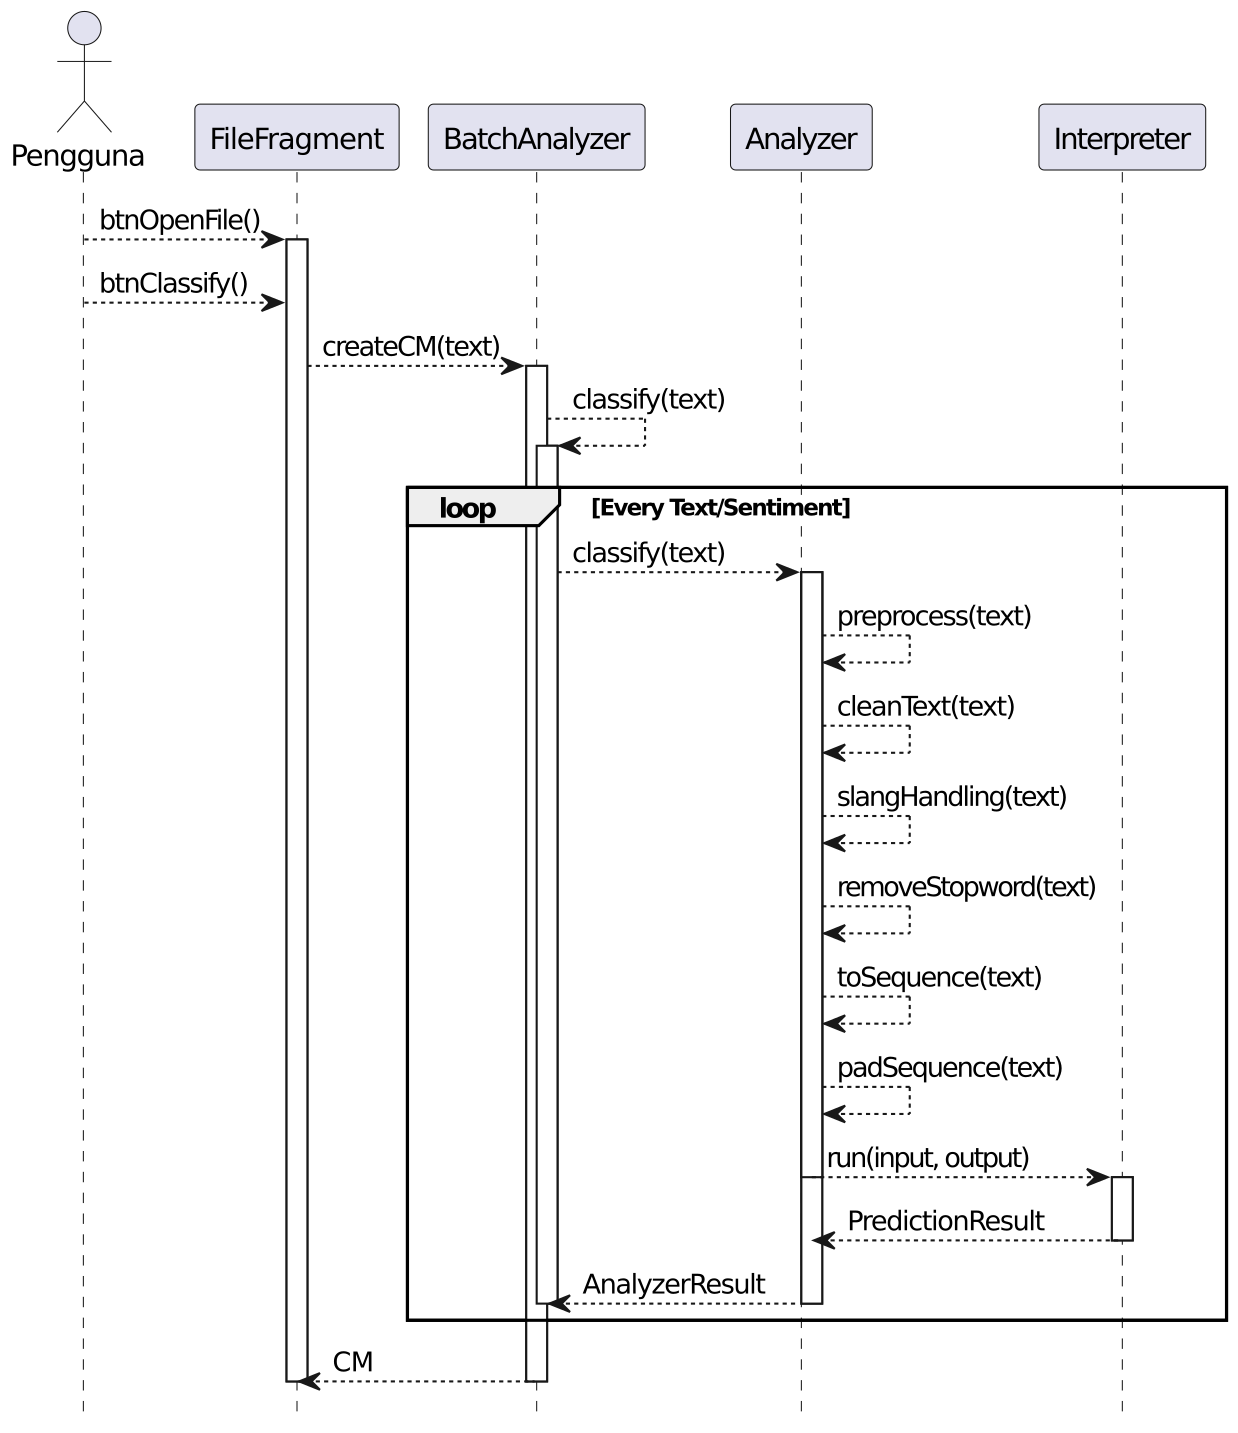
\includegraphics[width=\textwidth]{assets/sequence_diagram_file.png}
  \caption{Sequence Diagram File}
  \label{fig:sequence_diagram_file}
\end{figure}

\begin{figure}[H]
  \centering
  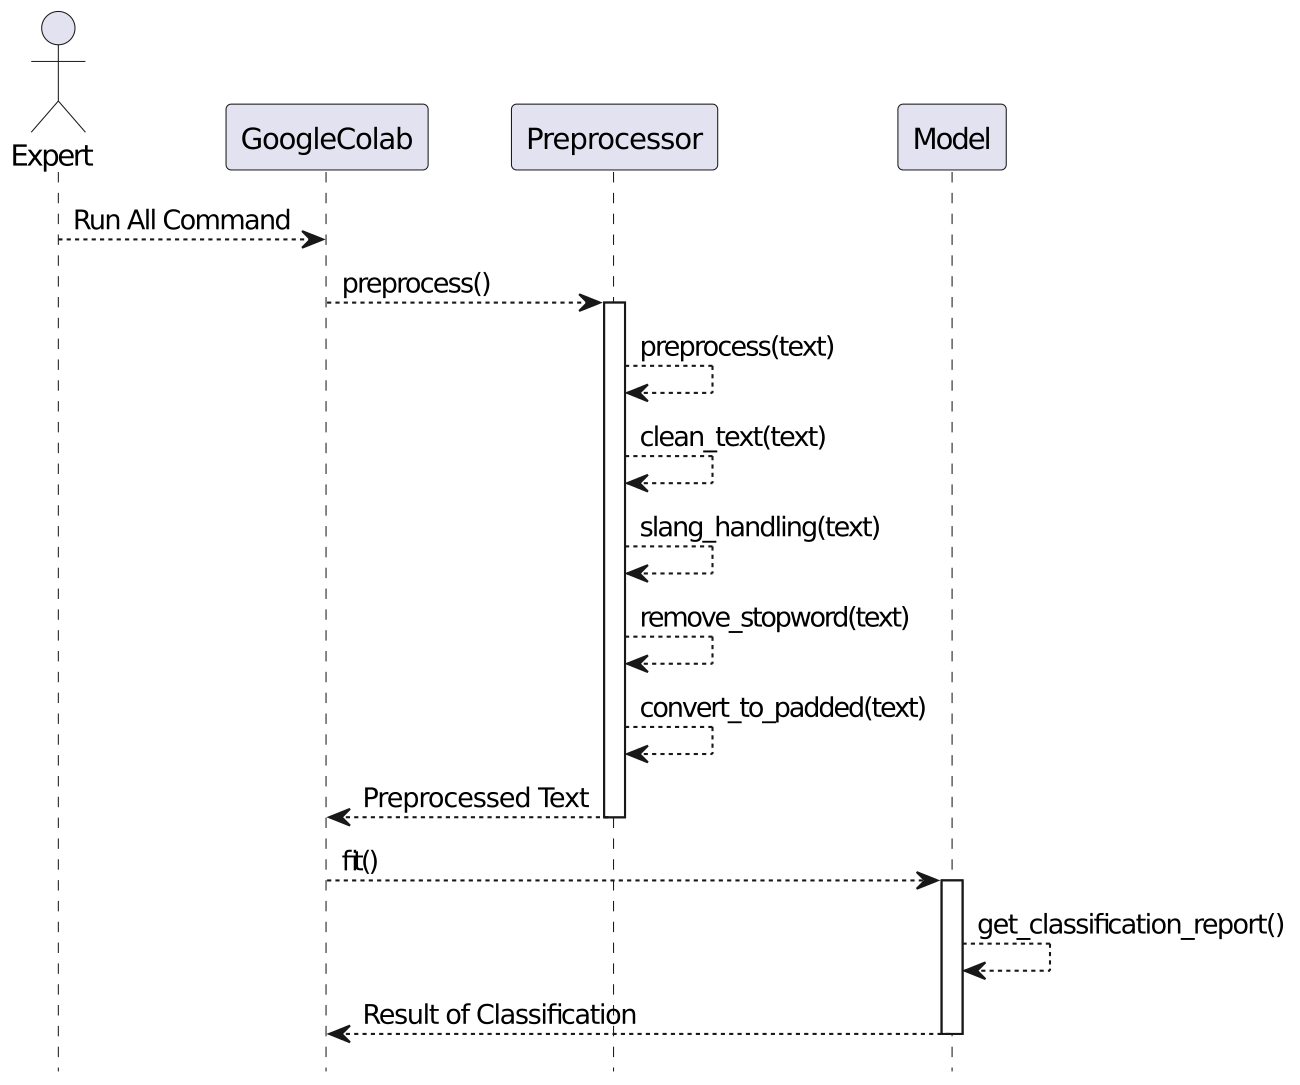
\includegraphics[width=\textwidth]{assets/sequence_diagram_test.png}
  \caption{Sequence Diagram Pengujian}
  \label{fig:sequence_diagram_test}
\end{figure}


\section{Fase Konstruksi}
Fase ketiga atau Fase Konstruksi dalam fase ini terdapat langkah-langkah yang harus dilakukan yaitu
pemodelan diagram kelas dan melakukan implementasi dari rancangan antarmuka (\emph{interface})
program dan diagram kelas.

\subsection{Diagram Kelas}
Diagram kelas atau umumnya dikenal sebagai diagram UML yang menjelaskan deksripsi, relasi, atribut, dan metode yang
ada dikelas dari perangkat lunak yang dikembangkan. Diagram kelas dapat dilihat pada
Gambar~\ref{fig:class_diagram_kalimat} dan pada Gambar~\ref{fig:class_diagram_file}.

\begin{figure}[H]
  \centering
  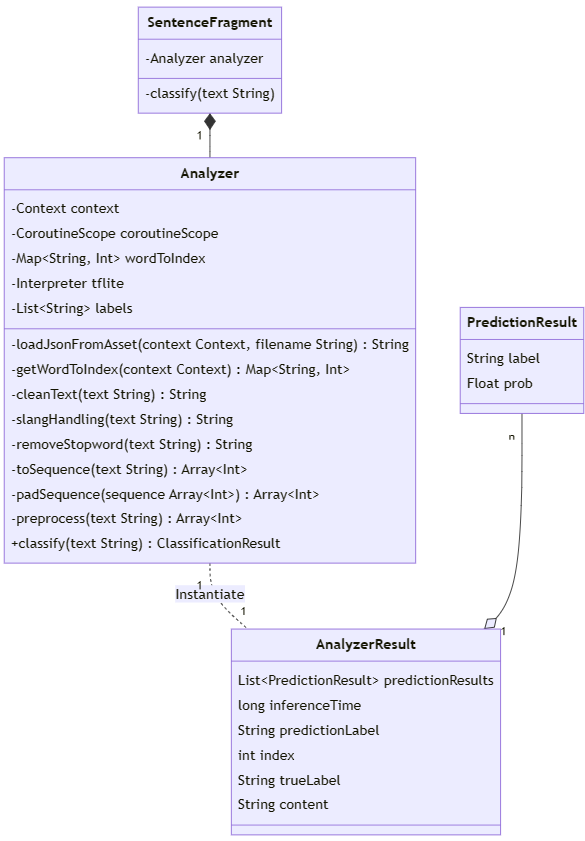
\includegraphics[scale=0.67]{assets/class_diagram_kalimat.png}
  \caption{Diagram Kelas Kalimat}
  \label{fig:class_diagram_kalimat}
\end{figure}

\begin{figure}[H]
  \centering
  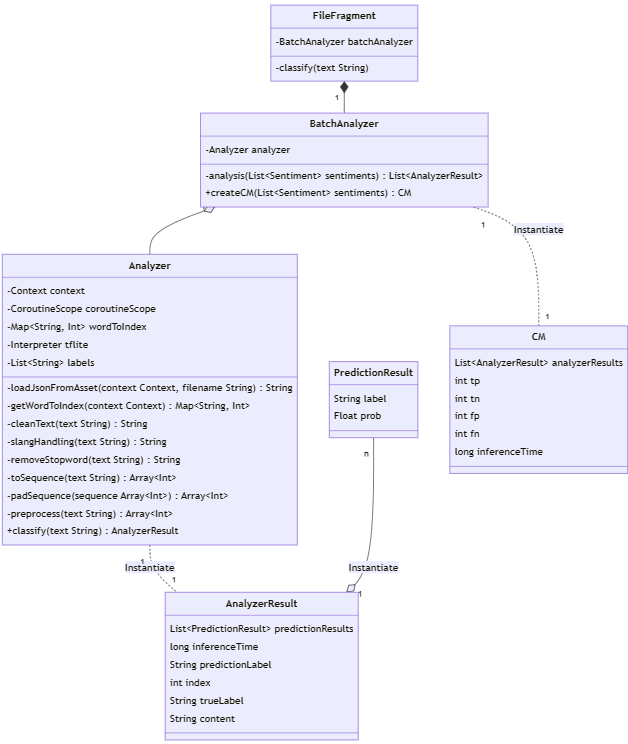
\includegraphics[width=\textwidth]{assets/class_diagram_file.png}
  \caption{Diagram Kelas File}
  \label{fig:class_diagram_file}
\end{figure}

\begin{figure}[H]
  \centering
  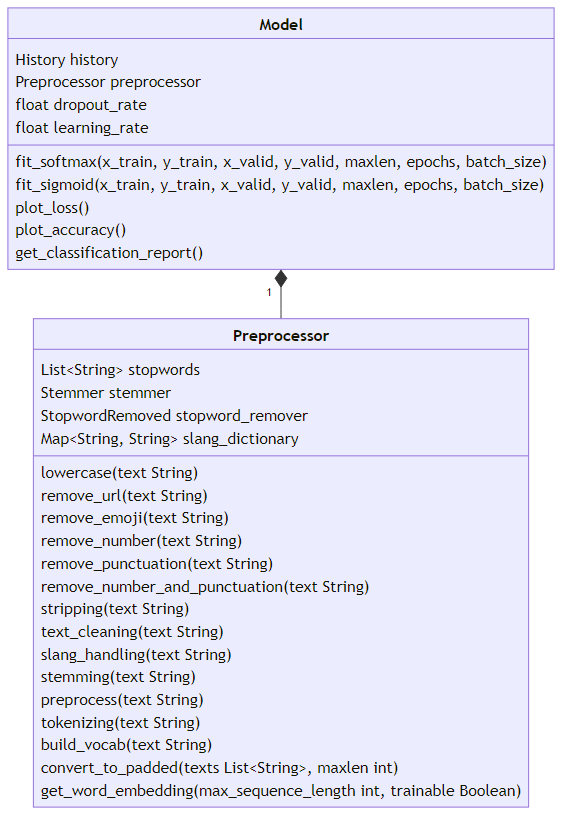
\includegraphics[scale=0.4]{assets/class_diagram_test.png}
  \caption{Diagram Kelas Pengujian}
  \label{fig:class_diagram_kalimat}
\end{figure}

\subsection{Implementasi Diagram Kelas}
Kelas yang telah dirancang dalam bentuk diagram kelas pada Gambar~\ref{fig:class_diagram_file} dan pada
Gambar~\ref{fig:class_diagram_kalimat} diimplementasikan pada program dengan
menggunakan bahasa pemrograman \emph{kotlin}. Pada Tabel~\ref{tab:class_implementation} adalah daftar
kelas yang sudah diimplementasikan ke dalam bentuk kode program.

\begin{longtable}[c]{|l|l|l|l|}
  \caption{Implementasi Diagram Kelas}
  \label{tab:class_implementation}                                                                                                                                                                                        \\
  \hline
  No                                                             &
  \multicolumn{1}{c|}{Nama Kelas}                                &
  \multicolumn{1}{c|}{Nama File}                                 &
  \multicolumn{1}{c|}{Keterangan}                                                                                                                                                                                         \\ \hline
  %
  \endhead
  \hline
  \endfoot
  %
  1                                                              &
  \begin{tabular}[c]{@{}l@{}}Sentence\\ Fragment\end{tabular}    &
  \begin{tabular}[c]{@{}l@{}}Sentence\\ Fragment.kt\end{tabular} &
  \begin{tabular}[c]{@{}l@{}}Kelas yang mengatur tampilan dan interaksi \\ dari fitur Analisis Sentimen Perkalimat\end{tabular}                                                                                           \\ \hline
  2                                                              &
  \begin{tabular}[c]{@{}l@{}}File\\ Fragment\end{tabular}        &
  \begin{tabular}[c]{@{}l@{}}File\\ Fragment.kt\end{tabular}     &
  \begin{tabular}[c]{@{}l@{}}Kelas yang mengatur tampilan dan \\ interaksi dari fitur Analisis Sentimen File\end{tabular}                                                                                                 \\ \hline
  3                                                              &
  \begin{tabular}[c]{@{}l@{}}Prediction\\ Result\end{tabular}    &
  \begin{tabular}[c]{@{}l@{}}Prediction\\ Result.kt\end{tabular} &
  \begin{tabular}[c]{@{}l@{}}Kelas yang menampung hasil dari prediksi \\ sentimen berupa label dan probabilitasnya\end{tabular}                                                                                           \\ \hline
  4                                                              &
  \begin{tabular}[c]{@{}l@{}}Analyzer\\ Result\end{tabular}      &
  \begin{tabular}[c]{@{}l@{}}Analyzer\\ Result.kt\end{tabular}   &
  \begin{tabular}[c]{@{}l@{}}Kelas yang menampung hasil dari prediksi \\ sentimen berapa lama proses prediksi untuk\\ satu sentimen, label yang diprediksi,\\ label yang asli,  index, dan kalimat sentimen.\end{tabular} \\ \hline
  5                                                              &
  \begin{tabular}[c]{@{}l@{}}CM\end{tabular}                     &
  \begin{tabular}[c]{@{}l@{}}CM.kt\end{tabular}                  &
  \begin{tabular}[c]{@{}l@{}}Kelas yang menampung hasil dari analisis\\ sentimen, true positive, true negative, false\\ positive,  false negative, dan berapa lama\\ proses analisis sentimen\end{tabular}                \\ \hline
  6                                                              &
  Sentiment                                                      &
  Sentiment.kt                                                   &
  \begin{tabular}[c]{@{}l@{}}Kelas yang menampung data sentimen\\ dari  file~.csv, berupa index, \\ kalimat sentiment,  dan labelnya\end{tabular}                                                                         \\ \hline
  8                                                              &
  \begin{tabular}[c]{@{}l@{}}Analyzer\end{tabular}               &
  \begin{tabular}[c]{@{}l@{}}Analyzer.kt\end{tabular}            &
  \begin{tabular}[c]{@{}l@{}}Kelas yang melakukan praproses dan \\ analisis  sentimen berdasarkan  kalimat\end{tabular}                                                                                                   \\ \hline
  9                                                              &
  \begin{tabular}[c]{@{}l@{}}Batch\\ Analyzer\end{tabular}       &
  \begin{tabular}[c]{@{}l@{}}Batch\\ Analyzer.kt\end{tabular}    &
  \begin{tabular}[c]{@{}l@{}}Kelas yang melakukan analisis sentiment \\ dari file~.csv dan menghasilkan \\ CM\end{tabular}                                                                                                \\ \hline
  10                                                             &
  \begin{tabular}[c]{@{}l@{}}Model\end{tabular}                  &
  \begin{tabular}[c]{@{}l@{}}model.py\end{tabular}               &
  \begin{tabular}[c]{@{}l@{}}Kelas yang melakukan pelatihan \\ dan pengujian analisis sentimen \\ dengan menggunakan CNN\end{tabular}                                                                                     \\ \hline
  11                                                             &
  \begin{tabular}[c]{@{}l@{}}Preprocessor\end{tabular}           &
  \begin{tabular}[c]{@{}l@{}}preprocessor.py\end{tabular}        &
  \begin{tabular}[c]{@{}l@{}}Kelas yang melakukan praproses pada data\end{tabular}                                                                                                                                        \\ \hline
\end{longtable}

\subsection{Implementasi Antarmuka (\emph{Interface}) Program}
\begin{figure}[H]
  \centering
  \fbox{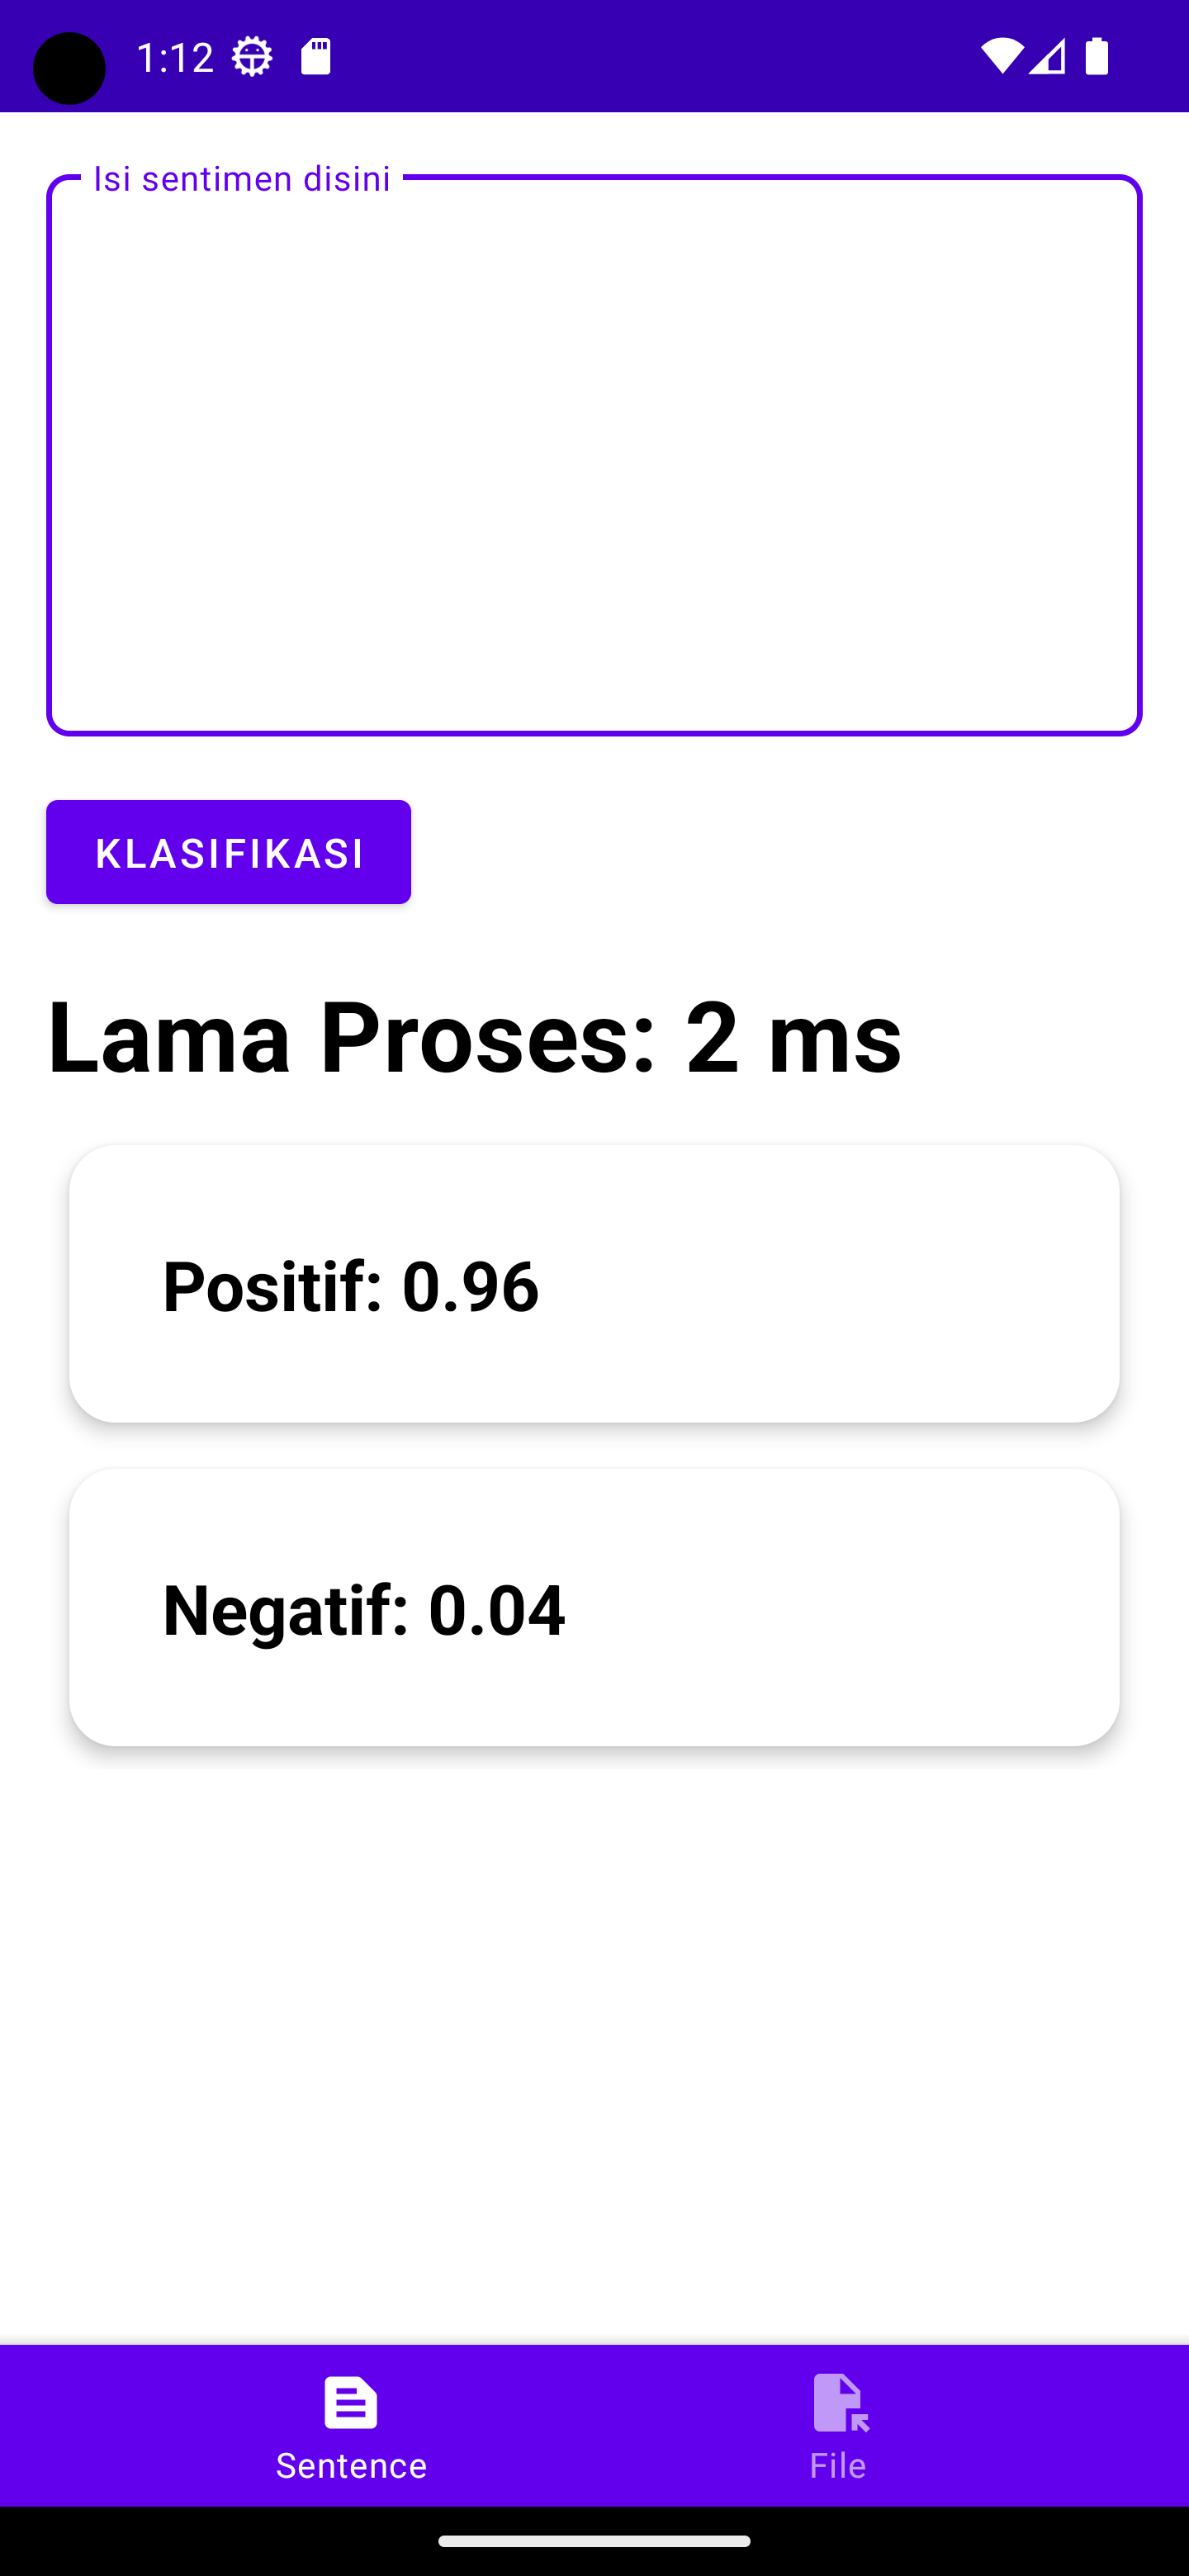
\includegraphics[width=8cm, height=9cm, keepaspectratio]{assets/interface_kalimat.png}}
  \caption{Implementasi Antarmuka Kalimat}
  \label{fig:interface_kalimat}
\end{figure}

\begin{figure}[H]
  \centering
  \fbox{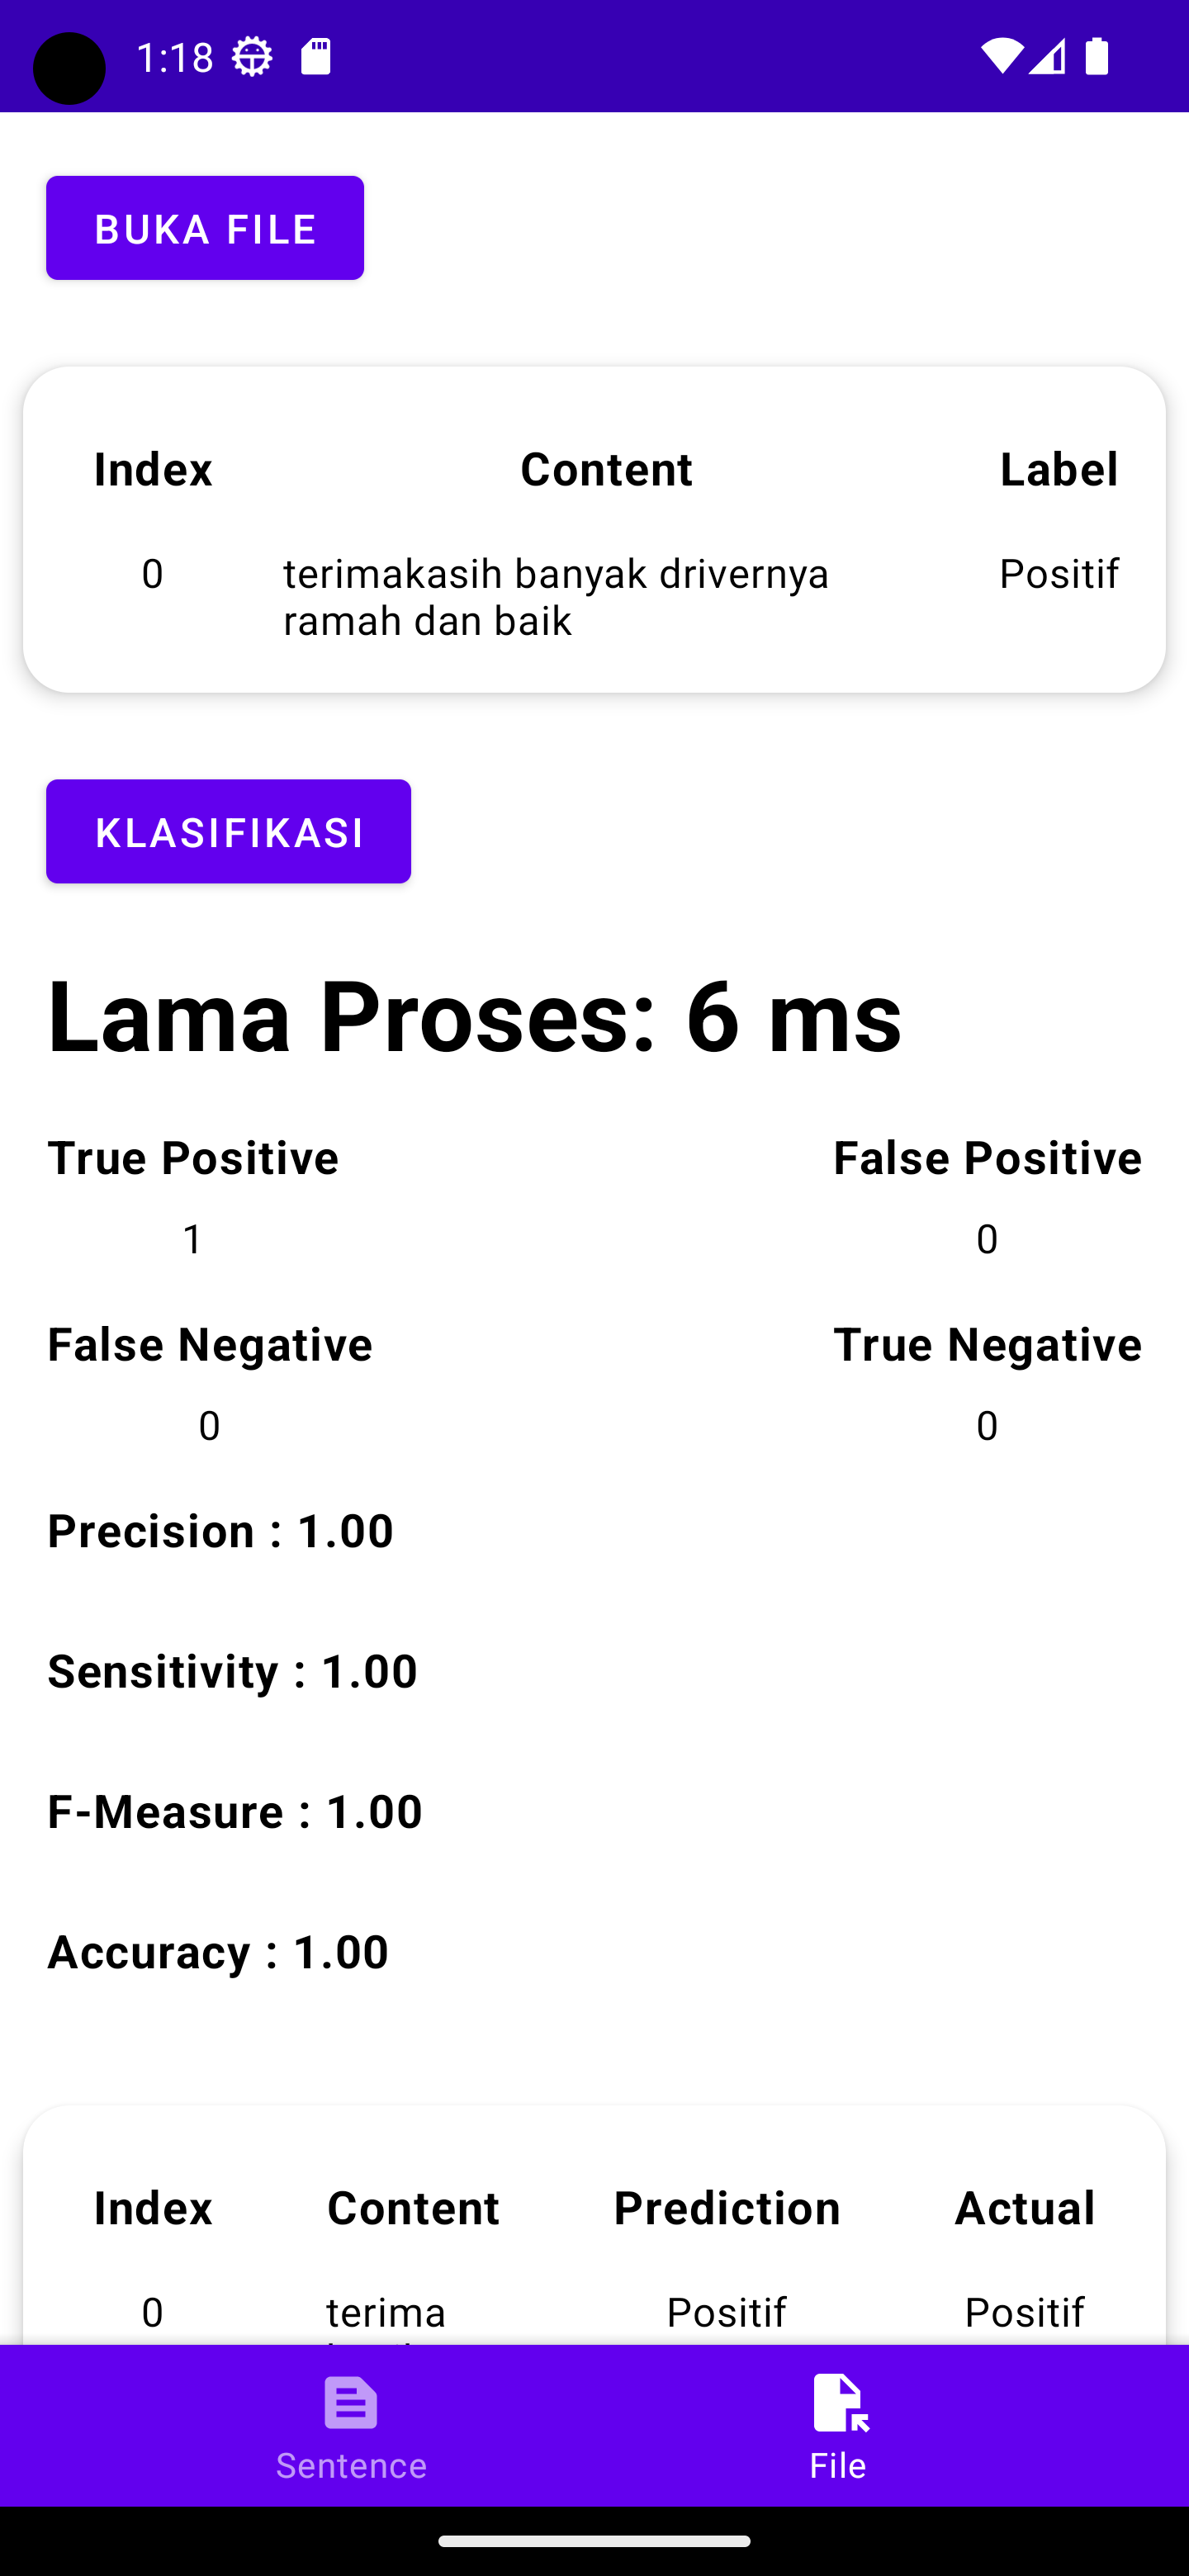
\includegraphics[width=8cm, height=9cm, keepaspectratio]{assets/interface_file.png}}
  \caption{Implementasi Antarmuka File}
  \label{fig:interface_file}
\end{figure}

\section{Fase Transisi}
Fase transisi merupakan fase terakhir dari metode pengembangan perangkat lunak RUP\@. Dalam fase perangkat
lunak diuji berdasarkan proses rencana pengujian untuk memastikan bahwa perangkat lunak dapat digunakan
sesuai dengan ekspektasi pengguna.

\subsection{Pemodelan Bisnis}
Dalam tahapan ini pengujian dilakukan dengan menggunakan cara \emph{black box testing} untuk menguji
apakah perangkat lunak yang dikembangkan berfungsi seperti yang diharapkan.

\emph{Black box testing} adalah cara pengujian dimana penguji tidak mengetahui bagaimana cara suatu sistem
bekerja, namun penguji hanya mengetahui masukan dan keluaran. Tujuan dari \emph{black box testing}
adalah untuk menguji fungsionalitas dari perangkat lunak apakah sudah sesuai dengan perencanaan yang telah dibuat
dan sudah sesuai dengan ekspektasi.

\subsection{Rencana Pengujian}
Rencana pengujian perangkat lunak dideskripsikan pada Tabel~\ref{tab:rencana_pengujian}

\begin{table}[H]
  \centering
  \caption{Rencana Pengujian}
  \label{tab:rencana_pengujian}
  \begin{tabularx}{\textwidth}{|l|X|X|X|c|}
    \hline
    No & \makecell[c]{Skenario                                                                                                                                                                                                                                     \\Pengujian} & \makecell[c]{Hasil yang\\Diharapkan} & \makecell[c]{Hasil\\Pengujian} & \makecell[c]{Kesimpulan} \\ \hline
    1  & Menekan tombol klasifikasi saat sudah menginput kalimat & Sistem menampilkan hasil klasifikasi berupa label dan probabilitasnya                      & Sistem menampilkan hasil klasifikasi berupa label dan probabilitasnya                      & Valid \\ \hline
    2  & Menekan tombol klasifikasi saat sudah membuka file~.csv & Sistem menampilkan hasil klasifikasi berupa index, kalimat, label dan label hasil prediksi & Sistem menampilkan hasil klasifikasi berupa index, kalimat, label dan label hasil prediksi & Valid \\ \hline
  \end{tabularx}
\end{table}

\section{Kesimpulan}
Pada bab ini telah dibahas tahapan yang dilakukan pada pengembangan perangkat lunak menggunakan metode
RUP untuk mengembangkan perangkat lunak yang digunakan sebagai alat bantu untuk melakukan penelitian.